\chapter{Introducción general}

Este capítulo pretende ser una guía general para el resto de capítulos. Se busca establecer el vocabulario y los conceptos necesarios para cualquier instrumento y medida que se tome.

\section{Glosario y vocabulario}

A continuación se enumera el vocabulario y las definiciones básicas que se requieren a lo largo del libro.

\begin{enumerate}
  \item Magnitud (\(X\)): se mide en la unidad física (\unit{\volt}, \unit{\ampere}, \unit{\ohm}). Usualmente en literatura ingenieril, se utiliza la letra \(U\) para hablar de diferencia de potencial (o tensión) como variable, \(I\) la corriente y \(R\) la resistencia.\footnote{Note que las unidades son rectas, mientras que las variables itálicas.}

  \item Exactitud: La proximidad del valor medido con el real.

  \item Precisión: La repetibilidad de las lecturas en el mismo. No siempre un instrumento preciso significa que sea exacto. A la inversa un instrumento exacto ha de ser siempre preciso.

  \item Sensibilidad de un instrumento: Relación efecto/causa. Esto se refiere puramente a la transferencia del dispositivo. Causa es la magnitud física que quiere medir (\(X\)). Por ejemplo: Tensión, Corriente o Temperatura. Efecto es la respuesta observable del instrumento (\(Y\)). Por ejemplo desplazamiento de la aguja en \unit{\milli\metre}.
    \[
      S_i = \frac{\Delta\text{Efecto}}{\Delta\text{Causa}} = \frac{\Delta Y}{\Delta X}
    \]
    Por ejemplo: tiene un termómetro de mercurio y por cada \qty{1}{\degreeCelsius} que sube la temperatura (causa), la columna de mercurio sube \qty{2}{\centi\metre} (efecto), la sensibilidad del instrumento es de \qty{2}{\centi\metre\per\degreeCelsius}.

    Si un instrumento (por ejemplo de imán permanente y bobina móvil) tiene una ley de respuesta
    \[
      I=k\alpha
    \]
    se puede ver claramente que para una pequeña variación de corriente \(\delta I\) habrá una pequeña variación de deflexión \(\delta\alpha\). Y a cada pequeño incremento de corriente le corresponderá el mismo cambio en la deflexión. Entonces se dice que la sensibilidad del instrumento es constante:
    \begin{equation}\label{eq_sensibilidad_constante}
      S=\frac{\delta \alpha}{\delta I}
    \end{equation}

    Por otro lado, si la deflexión responde a una ley alineal, entonces el cociente \eqref{eq_sensibilidad_constante} no es constante y varía punto a punto, donde su expresión matemática será 
    \[
      \lim_{\Delta I \to 0} \frac{\Delta \alpha}{\Delta I} \approx \frac{d\alpha}{dI}
    \]

  \item Sensibilidad de una técnica de medida: Se define como el cociente entre la magnitud total y el cambio más pequeño que es capaz de detectar. Por ejemplo si desea medir con un calibre muy sensible, pero lo utiliza para medir una pieza vibratoria o en un ambiente con muy mala iluminación, su capacidad para distinguir una pequeña variación disminuye. La \emph{técnica} se vuelve menos sensible aunque el instrumento siga siendo el mismo.
    
  \item Medir: Significa comparar una magnitud correspondiente con una unidad apropiada. El valor de la medida queda expresado como el producto entre el valor medido y la unidad correspondiente.

  \item Deflexión (\(\alpha\)): Cantidad de divisiones o grados que se desvía la aguja indicadora sobre una escala de un determinado instrumento. La deflexión suele ser un ángulo de giro o la cantidad de divisiones\footnote{Para la unidad no estándar ``divisiones'' que recorre la aguja de un instrumento cuando se deflexiona usaremos la unidad \unit{\div}.} que ha recorrido la aguja. Se denomina \(\alpha\) al valor actual en donde se detiene la aguja y \(\alpha_\text{max}\) al límite físico del instrumento (fondo de la escala).

    Un ejemplo: si tiene un voltímetro con una escala de \qtyrange{0}{50}{\div} y lo usa para medir en un rango de \qty{0}{\volt} a \qty{500}{\volt}, entonces \(\alpha_{\text{max}}=\qty{50}{\div}\).\footnote{Vea, que se dice \qtyrange{0}{50}{\div} ya que hay instrumentos que permiten deflexión hacia dos lados, de modo que, a modo de ejemplo, un voltímetro puede indicar \qtyrange{-25}{25}{\volt} y tener \qtyrange{-10}{10}{\div}.} Si al realizar una medida la aguja se clava a la mitad, la \emph{deflexión} es de \qty{25}{\div}, consecuentemente la lectura será de \qty{250}{\volt}.

  \item Campo nominal de referencia: Indica el \emph{rango} de un determinado parámetro en el cual el instrumento mantiene su clase (exactitud). Por ejemplo un voltímetro para corriente alterna que tiene una leyenda indicando \qtyrange{40}{60}{\hertz} quiere decir que su exactitud en la medida se mantiene siempre y cuando se respete ese rango de la frecuencia.

  \item Clase: se define como el error absoluto máximo \(E_{\text{max}}\) que puede cometer el instrumento en cualquier parte de su escala, referido a su alcance expresado en valor porcentual:
    \[
      c = \frac{E_{\text{max}}}{\text{Alcance}}\cdot 100
    \]
    La definición de alcance se presentará en las próximas definiciones.

  \item Cuadrante: es la cara frontal del instrumento que permite interpretar la magnitud medida. Contiene la escala graduada que es el conjunto de trazos y números que representan los valores de magnitud, la aguja indicadora (o índice) que se desplaza sobre el cuadrante para indicar el valor medido y un espejo antiparo que es una franja de espejo situada bajo la escala que sirve para evitar el error de paralaje.

    El cuadrante del instrumento puede contener un número acompañado con un símbolo indicando el principio de funcionamiento. Dicho número representa la clase del instrumento que, cuanto menor sea, mejor será la exactitud de las medidas. Si el instrumento no cuenta con el número de clase, el fabricante no garantiza la clase del instrumento.

  \item Rango de medida: Se define así al tramo de la escala en el cuadrante donde las medidas son confiables. 
    \[
      \text{Rango de medida} = [X_{\text{min}},X_{\text{max}}]
    \]
    El valor máximo del rango de medida (máxima magnitud: \(X_{\text{max}}\)) queda definido como el \emph{alcance} del instrumento. 

    Por ejemplo si se tiene un voltímetro que presenta en la escala del cuadrante \qty{0}{\volt} a \qty{500}{\volt} ese es su rango de medida (todos los valores entre \qtyrange{0}{500}{\volt}).

    Si el instrumento responde a una ley de deflexión lineal, entonces el rango de medida será coincidente con el alcance. Para instrumentos cuya ley de deflexión es cuadrática, la escala será lineal. De modo que el fabricante tratará (mediante dispositivos constructivos) de que sea así. No obstante, estos últimos aparatos suelen representar los primeros valores de la escala de forma comprimida, debido a la imposibilidad de su correcta calibración. Así, el alcance del instrumento no considera correctas (o con la exactitud dada por la clase) a los primeros valores más comprimidos. 

  \item Rango de deflexión: similar al rango de medida, pero relacionado a la deflexión. Se define como 
    \[\text{Rango de deflexión}=[\alpha_\text{min},\alpha_\text{max}]\]
    Así, corresponde a el movimiento que puede tener la aguja del instrumento sobre el cuadrante.

    No necesariamente el rango de deflexión y el rango de medida coinciden en su totalidad. Algunos instrumentos presentan un pequeño desborde al llegar a los límites de deflexión, garantizando ser precisos en el rango de medida.

  \item Margen de la indicación: Toda la escala del cuadrante.

  \item Constante de lectura: Se define como el cociente entre el alcance (\(X_{\text{max}}\)) y la máxima deflexión en divisiones (\(\alpha_{\text{max}}\)).
    \[
      C_E = \frac{\text{Alcance}}{\alpha_{max}}
    \]
    Cuando la aguja se deflexiona una cantidad \(\alpha\), la magnitud que está midiendo será:
    \[
      X_{\text{medido}} = \alpha \, C_E
    \]

  \item Consumo propio: Es la potencia absorbida por el propio instrumento para provocar su propia deflexión. Un voltímetro tendrá idealmente una resistencia infinita. Un amperímetro, idealmente, tendrá una resistencia nula. 

    Un voltímetro es conectado usualmente en paralelo\footnote{Recuerde que \(U\) representa la tensión.}. Así, su potencia de consumo será menor siempre que la resistencia sea mayor: \(P=\frac{U^2}{R}\). Para un amperímetro, que se conecta en serie, su potencia de consumo será menor siempre y cuando la resistencia sea menor: \(P=I^2R\).

  \item Resolución instrumental: es la variación de magnitud que provoca un mínimo cambio apreciable en la medición. Este valor suele valer desde \(1/5\) a \(1/10\) de división. Por ejemplo en un voltímetro con un rango de medida de \qtyrange{0}{500}{\volt} y \qty{50}{\div}, asumiendo que el voltímetro tiene una resolución instrumental de \(1/5\) entonces el mínimo cambio apreciable en la medición es de \qty{2}{\volt}.

  \item Sobrecarga: Es la máxima cantidad destructiva que tolera el instrumento sobre la máxima cantidad nominal (alcance).
    \[\text{Sobrecarga}=\frac{X_{\text{destructiva}}}{X_{\text{max}}}\]
    Si un voltímetro tiene un alcance de \qty{100}{\volt} y una sobrecarga del \(150\%\) significa que el voltímetro puede tolerar \qty{150}{\volt} sin destruirse.

\end{enumerate}

Con estas definiciones y vocabulario puede comenzar a interpretar conceptos fundamentales como las definiciones de las unidades de medida.

\section{Unidades de medida}

El sistema de unidades de medida que se prefiere utilizar es el denominado Sistema Internacional (SI)\footnote{Más sobre el SI en \url{https://es.wikipedia.org/wiki/Sistema_Internacional_de_Unidades}.}. La tabla \ref{tab_sistema_internacional} muestra las unidades elementales del sistema internacional.

\begin{table}[ht]
  \centering
  \begin{tabular}{lll}
    \toprule
    \textbf{Magnitud física} & \textbf{Nombre de la unidad} & \textbf{Símbolo} \\
    \midrule
    Longitud                 & metro                       & \unit{m}   \\
    Masa                     & kilogramo                   & \unit{kg}  \\
    Tiempo                   & segundo                     & \unit{s}   \\
    Corriente eléctrica      & amperio                     & \unit{A}   \\
    Temperatura              & kelvin                      & \unit{K}   \\
    Cantidad de sustancia    & mol                         & \unit{mol} \\
    Intensidad luminosa      & candela                     & \unit{cd}  \\
    \bottomrule
  \end{tabular}
  \caption{Unidades básicas del Sistema Internacional de Unidades (SI)}
  \label{tab_sistema_internacional}
\end{table}
A continuación se desarrollará conceptualmente la obtención de las unidades que se requieren.

La comprensión plena de las deducciones requiere nociones previas sobre el flujo de carga y el potencial eléctrico. Un desarrollo extenso de estos principios físicos fundamentales, así como de las leyes que rigen el campo eléctrico, se encuentra disponible en el recurso complementario \citetitle{f2elio} \parencite{f2elio}.

\subsection{Definición de Ampère}

El Ampère (o amperio) es la unidad de medida de la corriente eléctrica. La corriente eléctrica es el flujo de carga eléctrica a través de un conductor. En un circuito eléctrico, la corriente se define como la cantidad de carga eléctrica que pasa por unidad de área en un tiempo determinado. La unidad de medida de la corriente es el amperio (\unit{\ampere}), que equivale a un culombio por segundo (\unit{\coulomb\per\second}).\footnote{Cuando se habla de flujo de carga, la carga se asume como positiva, aunque luego en la realidad las cargas circundantes sean negativas. Esto se asume así en la mayoría de libros de Física y Electromagnetismo.}

\begin{tcolorbox}[
    sidebyside, sidebyside align=top, sidebyside gap=0.5cm,
    lower separated=false, lefthand width=0.6\textwidth,
    frame empty, colback=white, sharp corners, boxrule=0pt,
    left=0pt, right=0pt, top=0pt
  ]
  Cuando hablamos de \emph{flujo de carga} (\(\Phi_Q\)) nos referimos a la cantidad de carga que se mueve a través de una sección transversal del conductor en un tiempo determinado.

  Para definir la corriente con mayor precisión, suponga que las cargas tienen un movimiento perpendicular a una superficie \(A\), según se observa en la figura \ref{fig_current}. La corriente se define como la tasa a la cual circula la carga a través de la superficie. Si \(\Delta Q\) es la carga que pasa a través de la superficie \(A\) en un intervalo de tiempo \(\Delta t\), la corriente promedio \(I_{\text{prom}}\) se define como se muestra en la ecuación \eqref{eq_i_prom}.

  \tcblower
  \centering
  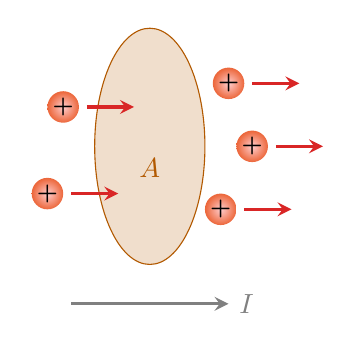
\begin{tikzpicture}[>=stealth]
  \draw[orange!70!black,fill=orange!70!black!20,name=conductor] (0,0) ellipse (0.7 and 1.5) node[below=0.8]{\(A\)};
  \draw[very thick,gray,->] (-1,-2) -- (1,-2) node[right]{\(I\)};

  \foreach \x\y in {-1.1/0.5,-1.3/-0.6,1/0.8,1.3/0,0.9/-0.8} {
    \shade[inner color=white!80!red, outer color=orange!50!red!70!lightgray] (\x,\y) node{\footnotesize\textbf{+}} circle (.2) [radius=1pt];
    \draw[very thick,color=red!70!gray,->] ({\x+0.3},\y) -- ({\x+0.9},\y);
  }

\end{tikzpicture}

  \captionsetup{hypcap=false} % Disable hycap for this fig
  \captionof{figure}{Cargas en movimiento a través de un área \(A\).}
  \label{fig_current}
\end{tcolorbox}
\begin{equation}\label{eq_i_prom}
  I_{\text{prom}} = \frac{\Delta Q}{\Delta t}
\end{equation}

Si la tasa a la que pasan las cargas varía en el tiempo, la corriente instantánea \(I\) se define como:
\[
  I = \lim_{\Delta t \to 0} \frac{\Delta Q}{\Delta t} = \frac{dQ}{dt}
\]
Para que exista un movimiento de cargas, es necesario que exista una fuerza que actúe sobre ellas. Esta fuerza es la fuerza eléctrica o ley de Coulomb, como muestra la ecuación \eqref{eq_coulomb}\footnote{En la ecuación \eqref{eq_coulomb} \(k_e=\qty{8.9876d9}{\newton\metre\squared\per\coulomb\squared}\) es la constante de Coulomb, \(q_1\) y \(q_2\) son las cargas y \(r\) es la distancia entre cargas.},
\begin{equation}\label{eq_coulomb}
  F=k_e \frac{\lvert q_1 \rvert \cdot \lvert q_2 \rvert}{r^2}
\end{equation}
Esta fuerza se manifiesta en un conductor en forma de campo eléctrico \(E\), que actúa sobre las cargas libres (electrones). Al provocar una diferencia de potencial\footnote{La diferencia de potencial es provocada mediante una reacción química (como en una batería), o mediante una fuente eléctrica.}, se crea este campo eléctrico que actúa sobre las cargas libres en el conductor. 

Cuando hay un campo eléctrico en un conductor, las cargas libres se aceleran y adquieren una velocidad. En palabras simples, podemos asociar la corriente eléctrica con el movimiento de cargas libres en un conductor.

En un conductor, los electrones libres se mueven en direcciones aleatorias debido a la temperatura del material. Sin embargo, cuando se aplica un campo eléctrico, estos electrones adquieren una velocidad de arrastre o velocidad de deriva \(v_d\) en la dirección del campo eléctrico. La velocidad de deriva es la velocidad promedio de las cargas (electrones en el caso de un conductor).
\begin{figure}[ht]
  \centering
  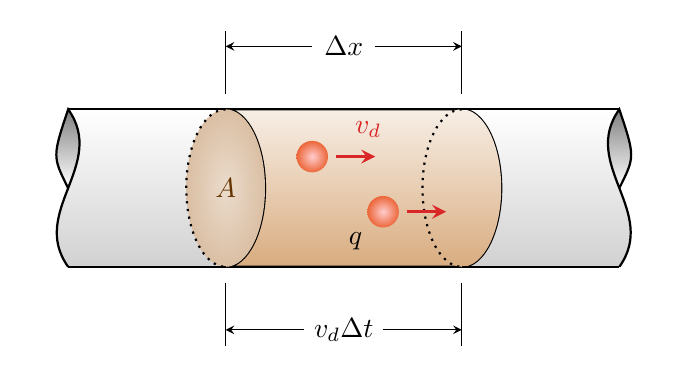
\begin{tikzpicture}[>=stealth]
    \def\rx{0.5}
    \def\ry{1}
    \def\lle{1.5}
    \def\curv{0.5}
    
    % Sombra conductor
    \shade[top color=orange!70!black!10, bottom color=orange!70!black!50] 
      (-\lle, \ry) -- (\lle, \ry)
      arc (90:-90:\rx cm and \ry cm)
      -- (-\lle, -\ry)
      arc (-90:90:\rx cm and \ry cm);

    % Sombra D (de corte)
    \shade (-\lle-2,0) .. controls (-\lle-2+\curv, 0.3) .. (-\lle-2, \ry) .. controls (-\lle-2-\curv+0.3, 0.4) .. (-\lle-2, 0);
    \shade (\lle+2,0) .. controls (\lle+2-\curv, 0.3) .. (\lle+2, \ry) .. controls (\lle+2+\curv-0.3, 0.4) .. (\lle+2, 0);

    % Sombra corte
    \shade[top color=white, bottom color=white!70!black!60] 
      (-\lle,-\ry) -- (-\lle-2,-\ry) .. controls (-\lle-2-\curv, -0.3) and (-\lle-2+\curv, 0.3) .. (-\lle-2, \ry) -- (-\lle,\ry);
    \shade[top color=white, bottom color=white!70!black!60] 
      (\lle,-\ry) -- (\lle+2,-\ry) .. controls (\lle+2+\curv, -0.3) and (\lle+2-\curv, 0.3) .. (\lle+2, \ry) -- (\lle,\ry);

    \draw[thick] 
      (-\lle, \ry) -- (\lle, \ry)
      arc (90:-90:\rx cm and \ry cm)
      -- (-\lle, -\ry)
      arc (-90:90:\rx cm and \ry cm);


    \shade[bottom color=orange!70!black!50, top color=orange!70!black!10] (\lle,0) ellipse (\rx cm and \ry cm);
    \shade[outer color=orange!60!black!36, inner color=orange!60!black!20] (-\lle,0) ellipse (\rx cm and \ry cm);

    % Sección de corte
    \draw[black,thick] (-\lle-2,-\ry) .. controls (-\lle-2-\curv, -0.3) and (-\lle-2+\curv, 0.3) .. (-\lle-2, \ry) .. controls (-\lle-2-\curv+0.3, 0.4) .. (-\lle-2, 0);
    \draw[black,thick] (\lle+2,-\ry) .. controls (\lle+2+\curv, -0.3) and (\lle+2-\curv, 0.3) .. (+\lle+2, \ry) .. controls (\lle+2+\curv-0.3, 0.4) .. (\lle+2, 0);
    \draw[black,thick] (-\lle,\ry) -- (-\lle-2,\ry);
    \draw[black,thick] (-\lle,-\ry) -- (-\lle-2,-\ry);
    \draw[black,thick] (\lle,\ry) -- (\lle+2,\ry);
    \draw[black,thick] (\lle,-\ry) -- (\lle+2,-\ry);

    \draw[thick, dotted] (-\lle,\ry) arc (90:270:\rx cm and \ry cm);
    \draw[thick, dotted] (\lle,\ry) arc (90:270:\rx cm and \ry cm);

    \node at (-\lle, 0) {\color{orange!40!black}\(A\)};

    % Cotas de medida
    \draw[thin] (-\lle,\ry+0.2) -- (-\lle,\ry+1);
    \draw[thin] (\lle,\ry+0.2) -- (\lle,\ry+1);
    \draw[thin,->] (-0.4,\ry+0.8) -- (-\lle,\ry+0.8);
    \draw[thin,->] (0.4,\ry+0.8) -- (\lle,\ry+0.8);
    \node at (0,\ry+0.8) {\(\Delta x\)};

    \draw[thin] (-\lle,-\ry-0.2) -- (-\lle,-\ry-1);
    \draw[thin] (\lle,-\ry-0.2) -- (\lle,-\ry-1);
    \draw[thin,->] (-0.5,-\ry-0.8) -- (-\lle,-\ry-0.8);
    \draw[thin,->] (0.5,-\ry-0.8) -- (\lle,-\ry-0.8);
    \node at (0,-\ry-0.8) {\(v_d \Delta t\)};

    % Cargas
    \shade[inner color=white!80!red, outer color=orange!50!red!70!lightgray] (-0.4,0.4) circle (.2) [radius=1pt];
    \draw[very thick,color=red!70!gray,->] (-0.1,0.4) node[above right=3pt] {\(v_d\)}-- (0.4,0.4) ;
    \shade[inner color=white!80!red, outer color=orange!50!red!70!lightgray] (0.5,-0.3) node[below left=4pt] {\(q\)} circle (.2) [radius=1pt];
    \draw[very thick,color=red!70!gray,->] (0.8,-0.3) -- (1.3,-0.3);
  \end{tikzpicture}
  \caption{Movimiento de cargas en un conductor.}
  \label{fig_movimiento_de_cargas}
\end{figure}


Recordando que \(\Delta Q\) es la cantidad de carga que pasa a través de la sección transversal \(A\), si toma un pedazo de conductor de longitud \(\Delta x\) como se muestra en la figura \ref{fig_movimiento_de_cargas}, puede expresar el volumen de este segmento de conductor como \(A\cdot\Delta x=A\cdot v_d\cdot \Delta t\). Si \(n\) es la densidad de cargas (número de cargas por unidad de volumen), el número de cargas en el segmento es \(nAv_d\Delta t\). Entonces la carga total de esa sección es
\begin{equation}\label{eq_carga_en_el_conductor}
  \Delta Q = (n\, A\, v_d\, \Delta t) q
\end{equation}
donde \(q\) es la carga de cada portador (electrones). Así se puede obtener la expresión de la corriente operando sobre la expresión \eqref{eq_carga_en_el_conductor}. Si divide ambos lados de la ecuación por \(\Delta t\) resulta
\begin{equation}\label{eq_corriente_promedio}
  I_\text{prom}=\frac{\Delta Q}{\Delta t} = n \, A\, v_d\, q
\end{equation}
que es la expresión de la corriente promedio.

\begin{figure}[ht]
  \centering
  \begin{subfigure}[b]{0.48\textwidth}
    \centering
    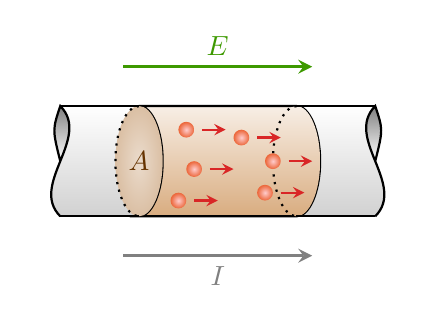
\begin{tikzpicture}[>=stealth]
      \def\rx{0.3}
      \def\ry{0.7}
      \def\lle{1}
      \def\cond{1}
      \def\curv{0.4}
      
      % Sombra conductor
      \shade[top color=orange!70!black!10, bottom color=orange!70!black!50] 
        (-\lle, \ry) -- (\lle, \ry)
        arc (90:-90:\rx cm and \ry cm)
        -- (-\lle, -\ry)
        arc (-90:90:\rx cm and \ry cm);

      % Sombra D (de corte)
      \shade (-\lle-\cond,0) .. controls (-\lle-\cond+\curv, 0.3) .. (-\lle-\cond, \ry) .. controls (-\lle-\cond-\curv+0.3, 0.4) .. (-\lle-\cond, 0);
      \shade (\lle+\cond,0) .. controls (\lle+\cond-\curv, 0.3) .. (\lle+\cond, \ry) .. controls (\lle+\cond+\curv-0.3, 0.4) .. (\lle+\cond, 0);

      % Sombra corte
      \shade[top color=white, bottom color=white!70!black!60] 
        (-\lle,-\ry) -- (-\lle-\cond,-\ry) .. controls (-\lle-\cond-\curv, -0.3) and (-\lle-\cond+\curv, 0.3) .. (-\lle-\cond, \ry) -- (-\lle,\ry);
      \shade[top color=white, bottom color=white!70!black!60] 
        (\lle,-\ry) -- (\lle+\cond,-\ry) .. controls (\lle+\cond+\curv, -0.3) and (\lle+\cond-\curv, 0.3) .. (\lle+\cond, \ry) -- (\lle,\ry);

      \draw[thick] 
        (-\lle, \ry) -- (\lle, \ry)
        arc (90:-90:\rx cm and \ry cm)
        -- (-\lle, -\ry)
        arc (-90:90:\rx cm and \ry cm);


      \shade[bottom color=orange!70!black!50, top color=orange!70!black!10] (\lle,0) ellipse (\rx cm and \ry cm);
      \shade[outer color=orange!60!black!36, inner color=orange!60!black!20] (-\lle,0) ellipse (\rx cm and \ry cm);

      % Sección de corte
      \draw[black,thick] (-\lle-\cond,-\ry) .. controls (-\lle-\cond-\curv, -0.3) and (-\lle-\cond+\curv, 0.3) .. (-\lle-\cond, \ry) .. controls (-\lle-\cond-\curv+0.3, 0.4) .. (-\lle-\cond, 0);
      \draw[black,thick] (\lle+\cond,-\ry) .. controls (\lle+\cond+\curv, -0.3) and (\lle+\cond-\curv, 0.3) .. (+\lle+\cond, \ry) .. controls (\lle+\cond+\curv-0.3, 0.4) .. (\lle+\cond, 0);
      \draw[black,thick] (-\lle,\ry) -- (-\lle-\cond,\ry);
      \draw[black,thick] (-\lle,-\ry) -- (-\lle-\cond,-\ry);
      \draw[black,thick] (\lle,\ry) -- (\lle+\cond,\ry);
      \draw[black,thick] (\lle,-\ry) -- (\lle+\cond,-\ry);

      \draw[thick, dotted] (-\lle,\ry) arc (90:270:\rx cm and \ry cm);
      \draw[thick, dotted] (\lle,\ry) arc (90:270:\rx cm and \ry cm);

      \node at (-\lle, 0) {\color{orange!40!black}\(A\)};

      % Dirección de la corriente convencional
      \draw[very thick, gray, ->] (-\lle-0.2,-\ry-0.5) -- node[below]{\(I\)} (\lle+0.2,-\ry-0.5);
      % Dirección del campo eléctrico
      \draw[very thick, green!60!yellow!60!black, ->] (-\lle-0.2,\ry+0.5) -- node[above]{\(E\)} (\lle+0.2,\ry+0.5);

      % Cargas
      \foreach \x\y in {-0.4/0.4,-0.3/-0.1,-0.5/-0.5,0.3/0.3,0.7/0,0.6/-0.4} {
        \shade[inner color=white!80!red, outer color=orange!50!red!70!lightgray] (\x,\y) circle (.1) [radius=1pt];
        \draw[thick,color=red!70!gray,->] (\x+0.2,\y) -- (\x+0.5,\y) ;
      }
    \end{tikzpicture}
    \caption{Una corriente convencional es tratada como un flujo de cargas positivas, sin importar si las cargas libres del conductor son positivas, negativas o ambas.}
    \label{fig:flujo_de_cargas_positivas}
  \end{subfigure}
  \hfill
  \begin{subfigure}[b]{0.48\textwidth}
    \centering
    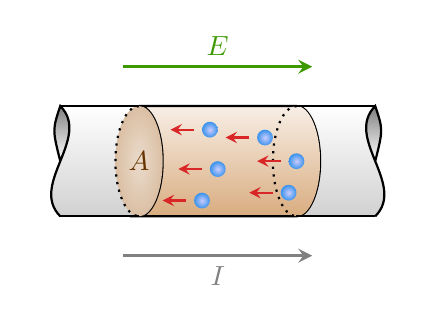
\begin{tikzpicture}[>=stealth]
      \def\rx{0.3}
      \def\ry{0.7}
      \def\lle{1}
      \def\cond{1}
      \def\curv{0.4}
      
      % Sombra conductor
      \shade[top color=orange!70!black!10, bottom color=orange!70!black!50] 
        (-\lle, \ry) -- (\lle, \ry)
        arc (90:-90:\rx cm and \ry cm)
        -- (-\lle, -\ry)
        arc (-90:90:\rx cm and \ry cm);

      % Sombra D (de corte)
      \shade (-\lle-\cond,0) .. controls (-\lle-\cond+\curv, 0.3) .. (-\lle-\cond, \ry) .. controls (-\lle-\cond-\curv+0.3, 0.4) .. (-\lle-\cond, 0);
      \shade (\lle+\cond,0) .. controls (\lle+\cond-\curv, 0.3) .. (\lle+\cond, \ry) .. controls (\lle+\cond+\curv-0.3, 0.4) .. (\lle+\cond, 0);

      % Sombra corte
      \shade[top color=white, bottom color=white!70!black!60] 
        (-\lle,-\ry) -- (-\lle-\cond,-\ry) .. controls (-\lle-\cond-\curv, -0.3) and (-\lle-\cond+\curv, 0.3) .. (-\lle-\cond, \ry) -- (-\lle,\ry);
      \shade[top color=white, bottom color=white!70!black!60] 
        (\lle,-\ry) -- (\lle+\cond,-\ry) .. controls (\lle+\cond+\curv, -0.3) and (\lle+\cond-\curv, 0.3) .. (\lle+\cond, \ry) -- (\lle,\ry);

      \draw[thick] 
        (-\lle, \ry) -- (\lle, \ry)
        arc (90:-90:\rx cm and \ry cm)
        -- (-\lle, -\ry)
        arc (-90:90:\rx cm and \ry cm);


      \shade[bottom color=orange!70!black!50, top color=orange!70!black!10] (\lle,0) ellipse (\rx cm and \ry cm);
      \shade[outer color=orange!60!black!36, inner color=orange!60!black!20] (-\lle,0) ellipse (\rx cm and \ry cm);

      % Sección de corte
      \draw[black,thick] (-\lle-\cond,-\ry) .. controls (-\lle-\cond-\curv, -0.3) and (-\lle-\cond+\curv, 0.3) .. (-\lle-\cond, \ry) .. controls (-\lle-\cond-\curv+0.3, 0.4) .. (-\lle-\cond, 0);
      \draw[black,thick] (\lle+\cond,-\ry) .. controls (\lle+\cond+\curv, -0.3) and (\lle+\cond-\curv, 0.3) .. (+\lle+\cond, \ry) .. controls (\lle+\cond+\curv-0.3, 0.4) .. (\lle+\cond, 0);
      \draw[black,thick] (-\lle,\ry) -- (-\lle-\cond,\ry);
      \draw[black,thick] (-\lle,-\ry) -- (-\lle-\cond,-\ry);
      \draw[black,thick] (\lle,\ry) -- (\lle+\cond,\ry);
      \draw[black,thick] (\lle,-\ry) -- (\lle+\cond,-\ry);

      \draw[thick, dotted] (-\lle,\ry) arc (90:270:\rx cm and \ry cm);
      \draw[thick, dotted] (\lle,\ry) arc (90:270:\rx cm and \ry cm);

      \node at (-\lle, 0) {\color{orange!40!black}\(A\)};

      % Dirección de la corriente convencional
      \draw[very thick, gray, ->] (-\lle-0.2,-\ry-0.5) -- node[below]{\(I\)} (\lle+0.2,-\ry-0.5);
      % Dirección del campo eléctrico
      \draw[very thick, green!60!yellow!60!black, ->] (-\lle-0.2,\ry+0.5) -- node[above]{\(E\)} (\lle+0.2,\ry+0.5);

      % Cargas
      \foreach \x\y in {-0.1/0.4,0/-0.1,-0.2/-0.5,0.6/0.3,1/0,0.9/-0.4} {
        \shade[inner color=white!80!blue, outer color=cyan!50!blue!70!lightgray] (\x,\y) circle (.1) [radius=1pt];
        \draw[thick,color=red!70!gray,->] (\x-0.2,\y) -- (\x-0.5,\y) ;
      }
    \end{tikzpicture}
    \caption{En un conductor metálico, las cargas en movimiento son electrones, pero la corriente aún apunta en la dirección en que fluirían las cargas positivas.}
    \label{fig:flujo_de_cargas_negativas}
  \end{subfigure}
  \caption{Movimiento de cargas en un conductor.}
  \label{fig_corriente_convencional}
\end{figure}


La figura \ref{fig_corriente_convencional} presenta segmentos de material conductor. En la figura \ref{fig:flujo_de_cargas_positivas}, las cargas en movimiento son positivas, la fuerza eléctrica ocurre en la misma dirección que \(E\), y la velocidad de deriva \(v_d\) es de izquierda a derecha. En la figura \ref{fig:flujo_de_cargas_negativas} las cargas son negativas, la fuerza eléctrica es opuesta a \(E\), y la velocidad de deriva \(v_d\) es de derecha a izquierda. Definimos que la corriente, denotada por \(I\), va en la dirección en la que hay un flujo de carga positiva. Por ello, las corrientes se describen como si consistieran por completo en un flujo de cargas positivas, aun en los casos en que se sabe que la corriente real se debe a electrones. Así, en las figuras \ref{fig:flujo_de_cargas_positivas} y \ref{fig:flujo_de_cargas_negativas} la corriente es hacia la derecha. Esta convención sobre la dirección del flujo de la corriente se llama \emph{corriente convencional}. Aunque la dirección de la corriente convencional no es necesariamente la misma en que se desplazan en realidad las partículas con carga, veremos que el signo de las cargas en movimiento tiene poca importancia en el análisis de los circuitos eléctricos.

La ecuación \eqref{eq_corriente_promedio} muestra una expresión para el cálculo de la corriente promedio en un intervalo de tiempo dado. Así, el amperio se deriva de \unit{\coulomb\per\second} (Coulomb por segundo) pero, ¿qué significa esto en términos fundamentales?

Desde la redefinición del SI en 2019, la unidad se basa en valores fijos de constantes naturales. Se fija la carga elemental (la carga de un electrón) exactamente en:
\begin{equation}
    e = \qty{1.602176634d-19}{\coulomb}
\end{equation}

Para comprender la magnitud de un amperio, podemos invertir esta relación para determinar cuántas cargas elementales constituyen un Coulomb:
\begin{align*}
    \qty{1}{\coulomb} &= \frac{1}{1.602176634\times 10^{-19}} e \\
    \qty{1}{\coulomb} &\approx \qty{6.241509d18}{} \text{ cargas elementales}
\end{align*}
Por lo tanto, sustituyendo esto en la definición de corriente ($I = q/t$), un amperio queda definido formalmente como:
\begin{equation}
    \qty{1}{\ampere} = \frac{\qty{1}{\coulomb}}{\qty{1}{\second}} \approx \frac{\qty{6.2415d18}{} \text{ electrones}}{\qty{1}{\second}}
\end{equation}
O, dicho de otra forma más fundamental: un amperio es el flujo de aproximadamente \num{6.2415d18} cargas elementales por segundo a través de una sección transversal determinada.

\subsubsection{Evolución del estándar: De la fuerza al flujo}

Es fundamental distinguir entre la definición histórica, que rigió la metrología durante gran parte del siglo XX, y la definición moderna basada en constantes fundamentales.

Anteriormente, el amperio se definía mediante un experimento idealizado de fuerza magnética. Se basaba en la Ley de Ampère para la fuerza entre dos conductores paralelos:
\begin{equation}
    \frac{F}{L} = \frac{\mu_0 I_1 I_2}{2\pi d}
\end{equation}
Para que esta definición fuera válida, el Sistema Internacional fijaba el valor exacto de la permeabilidad magnética del vacío en \(\mu_0 = 4\pi \times10^{-7}\unit{\henry\per\meter}\). Así, si la distancia \(d\) era \qty{1}{\meter} y la fuerza resultante era \qty{2d-7}{\newton} por metro, la corriente se definía como \qty{1}{\ampere}.

Esta definición dependía de una configuración geométrica ideal (cables infinitos, sección despreciable) difícil de replicar con alta precisión en un laboratorio.

La redefinición eliminó la dependencia de la geometría y la fuerza mecánica. Ahora, el amperio se define fijando la carga elemental \(e\) (un contador de partículas) y el segundo (basado en el reloj atómico de cesio).

Al fijar la carga elemental \(e\) como exacta, la permeabilidad del vacío \(\mu_0\) dejó de ser una constante exacta. En el sistema actual, \(\mu_0\) es un valor que debe determinarse experimentalmente, con una incertidumbre asociada (proporcional a la constante de estructura fina \(\alpha\)).

\subsection{Definición de Voltio}


